\documentclass[a4paper,12pt]{IEEEtran}
\usepackage{graphicx}
\usepackage[greek,english]{babel}
\graphicspath{{./report_plots/}}
\begin{document}

\title{CSC 510 Assignment 2 Report}
\author{Justin Oakley}
\maketitle\

\pagenumbering{arabic}
\tableofcontents
\newpage

\section{Introduction}
This report is about knowing machine learning techniques that will help in selecting suitable techniques which will provide excellent quality results for applications using the computing environment utilized in an experiment. The reason for why understanding these methods are so important in big data is because they provide higher quality data not only for machines to processes, but also for them to produce. The steps taken in order to obtain the desired data output are based on the type of learning that the machine must go through and the appropriate selection of models and algorithms that follow with that type of learning. In this assignment, supervised learning is the main type of learning that will be focused upon and the modeling strategies that will be heavily utilized in data analyzation are regression and classification.

As for the information that was processed, five different datasets were used in this assignment; one computer-generated dataset of fifty observations alongside two datasets based on recent graduate students (ages < 28) and graduate students (ages 25+), called \textit{recent-grads.csv} and \textit{grad-students.csv}, are experimented on in the regression model section, and two datasets about captured network normal and attack traffic, named \textit{nslkdd-version1.csv} and \textit{nslkdd-version2.csv}, are utilized in the classification portion. All data analyzation for the assignment is coded in the Python 3 language via the Apache Spark 2.4.0 computational engine on an Apache Hadoop cluster. With this in mind, the goal of the comprehending supervised machine learning techniques through model and algorithm selection can be achieved.

\section{Comparison of Regression Models}
The first step in developing a working knowledge of the functionality of machine learning techniques, such as regression, is to understand the significance of regression. Regression modeling is about predicting values based on the actual responses of \textit{y} and the domain values of \textit{x} being utilized in the processes of an error factor minimization and regularization to paramterize the model:  \[\textit{y} = \textit{A}\textbf{x}' - \textit{b}\] In order to accurately predict values using regression, the optimization process must take place, which means that several different models must be parametrized and compared together to see which has the lower error factor.

For this experiment, four different types of regression were performed on a generated dataset of fifty observations and the \textit{recent-grads.csv} and \textit{grad-students.csv} files. The three datasets where processed through all four types of regression to find the optimal parameters needed to make the most accurate predictions and the best fitting line or hyperplane. The four regression models used in this portion of the assignment were standard regression, ridge regression, lasso regression, and elastic-net regression. In the following subsections, each dataset's regression models will be compared and contrasted together, respectively.

\subsection{Generated Set of Points}
\label{gen_set}
In standard regression, the estimated parameter is found by calculating: \[\textit{A} = \textit{y}\textbf{x}'(\textbf{x}\textbf{x}')^{-1}\] then plugging the matrix \textit{A} into the model equation. When using the one-dimensional domain formed by the generated set of points was applied this algorithm, the following figure spawned: 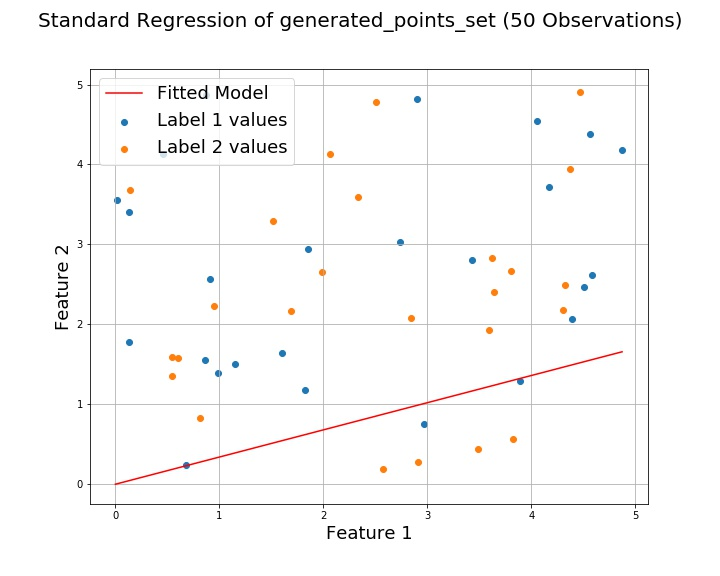
\includegraphics[width=8cm]{std_reg_1d_generated_points_set} while the two-dimensional domain of the dataset resulted in: 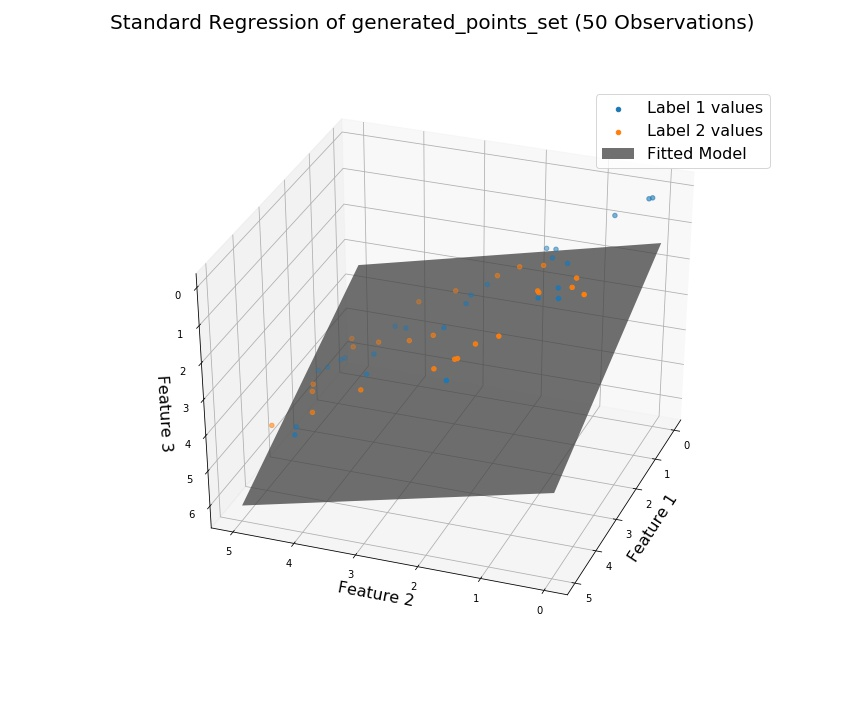
\includegraphics[width=9cm]{std_reg_2d_generated_points_set} Following the plotting of these graphs, the mean-squared error and the root-mean-squared error was calculated to be 0.22 and 0.46.

Now in the processing of the ridge regression model, where the regularization parameter is $\lambda \textit{a}^{2}$ which gives the estimate for the vector (matrix) model is
$$\textit{A} = \textit{y}\textbf{x}'(\textbf{x}\textbf{x}' + \lambda \textit{I})^{-1}$$the following plots were created from one-dimensional domain and the two-dimensional domain of the dataset: 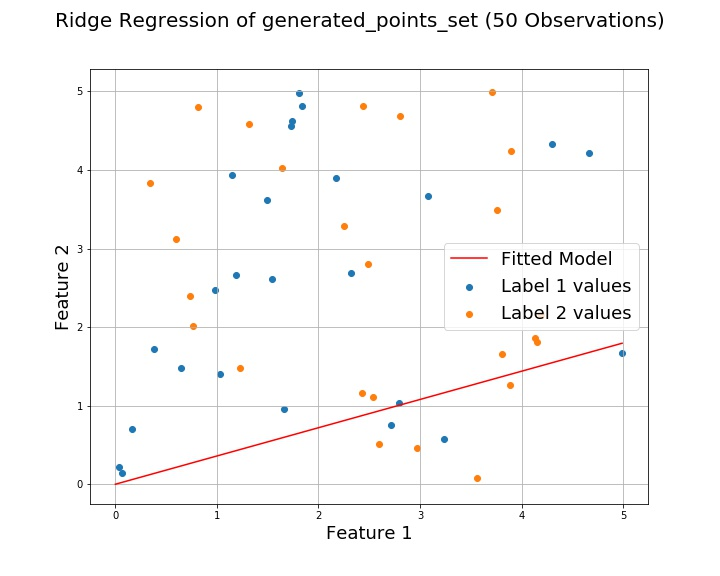
\includegraphics[width=8cm]{ridge_reg_1d_generated_points_set} 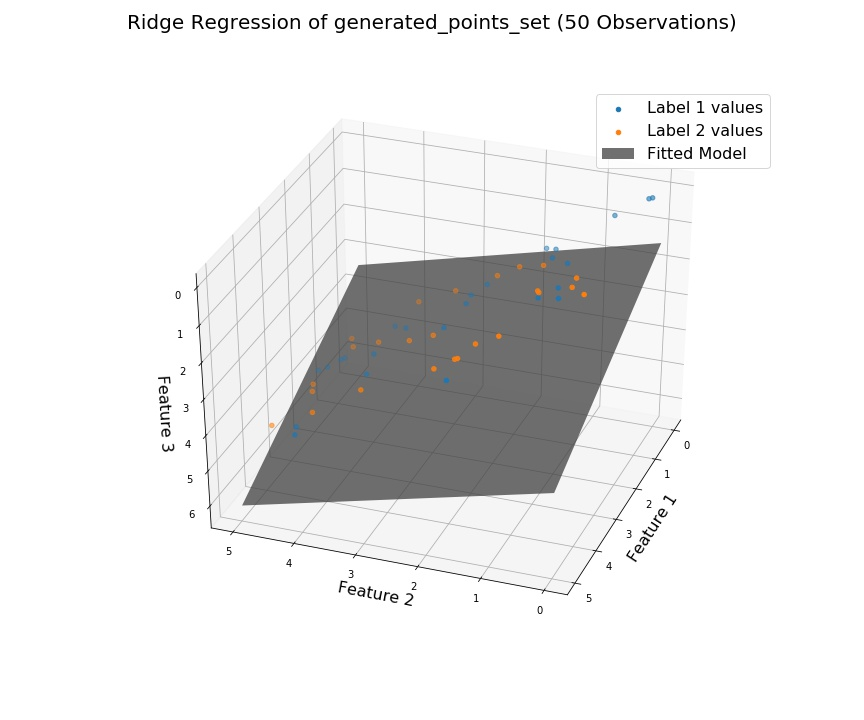
\includegraphics[width=9cm]{ridge_reg_2d_generated_points_set} and its mean-squared and root-mean-squared errors were 0.22 and 0.46. When comparing the two regression models together, the line of best fit does not appear to change in slope value, at least visually, and the both error values are the same as the standard regression error values. This means that a change in regression parameters does not effect the response variable \textit{Y}.

As for the lasso regression model, which is $$\textit{A} = (\textit{y}\textbf{x}' - \frac{\lambda}{2})\textbf{s})(\textbf{x}\textbf{x}')^{-1}$$,using the generated set of points' one-dimensional domain and two-dimensional domain, the plots came out to be 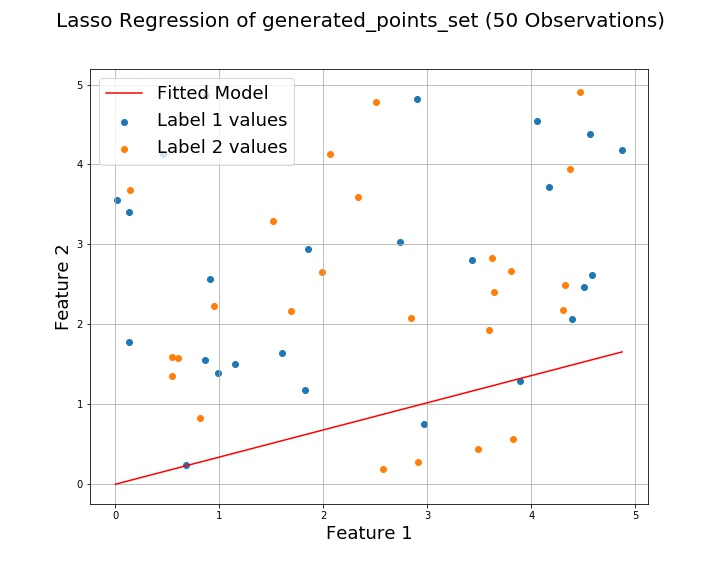
\includegraphics[width=8cm]{lasso_reg_1d_generated_points_set} 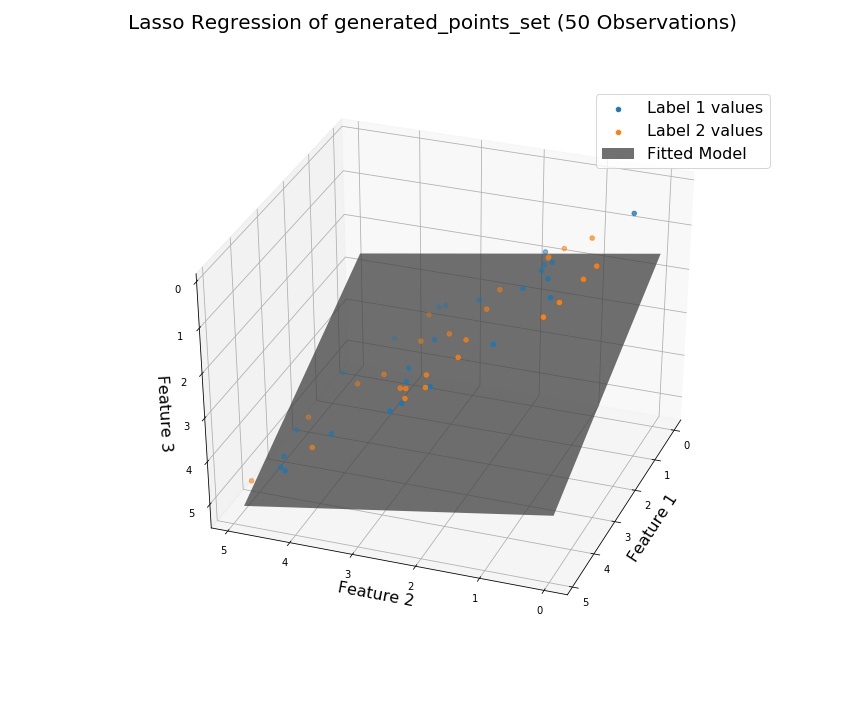
\includegraphics[width=9cm]{lasso_reg_2d_generated_points_set} with a mean-squared error of about 0.22 and a root-mean-squared error of about 0.46. Notice that still the change in parameters does not visually effect the regression line and regression plane nor dramatically effect the error values, meaning that continuing to add certain regularization parameters to the error factor does not affect the model.

Finally, the last regression model in the optimization process is the elastic-net regression technique. Elastic-net regression uses both regularization parameters (that were previously used in ridge and lasso regression) to form the estimate: $$\textit{A} = (\textit{y}\textbf{x}' - \frac{\lambda_{2}}{2})\textbf{s})(\textbf{x}\textbf{x}' +\lambda_{1} \textit{I})^{-1}$$ When the domains formed from the generated set of points are used using this type of modelling, they are visualized as such: 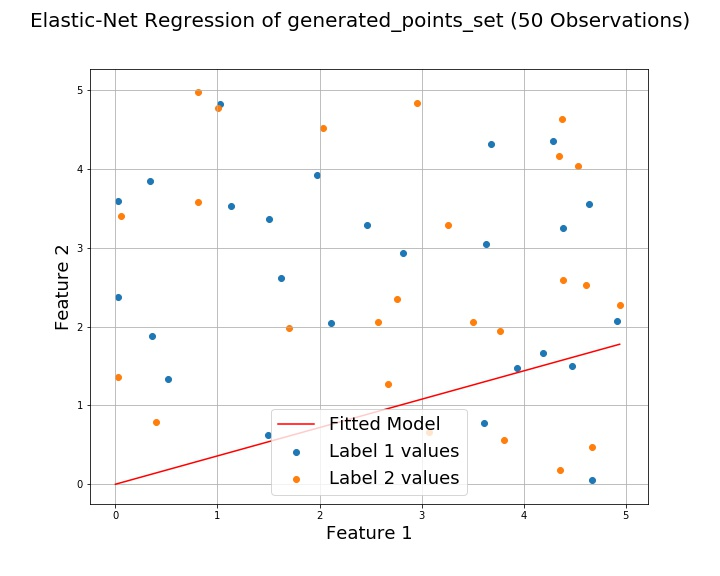
\includegraphics[width=8cm]{en_reg_1d_generated_points_set} 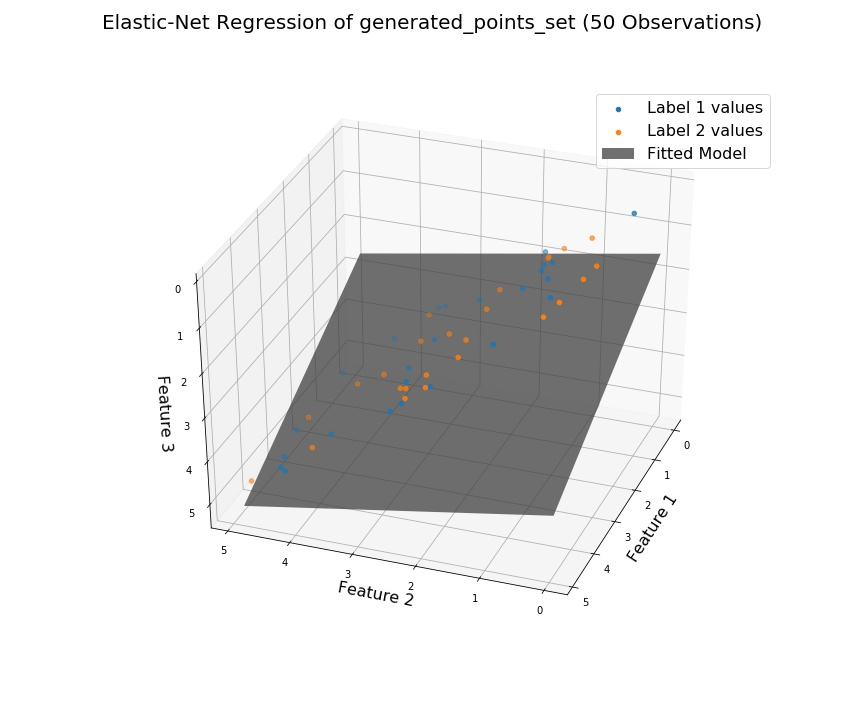
\includegraphics[width=9cm]{en_reg_2d_generated_points_set} and appear to have error values approximately the same as the previous three models' values. Again, there seems to be no distinguishable difference in each type of regression. This means that the generated set of points has an optimized model regardless of whatever type of regression would be used on the dataset.

\subsection{Recent Graduate Dataset}
\label{recent_grad}
Using the same type of parameters used in standard and ridge regression, the dataset containing information about recent graduate students resulted in the following plots featuring the line of best fit. 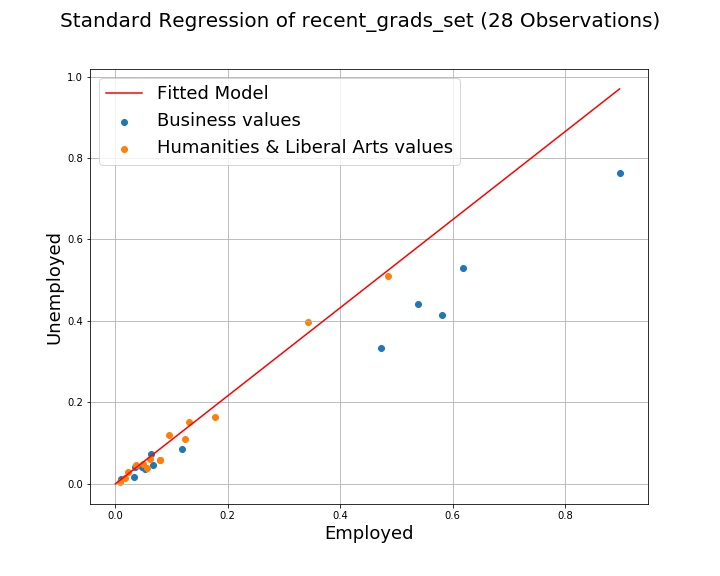
\includegraphics[width=8cm]{std_reg_1d_recent_grads_set} 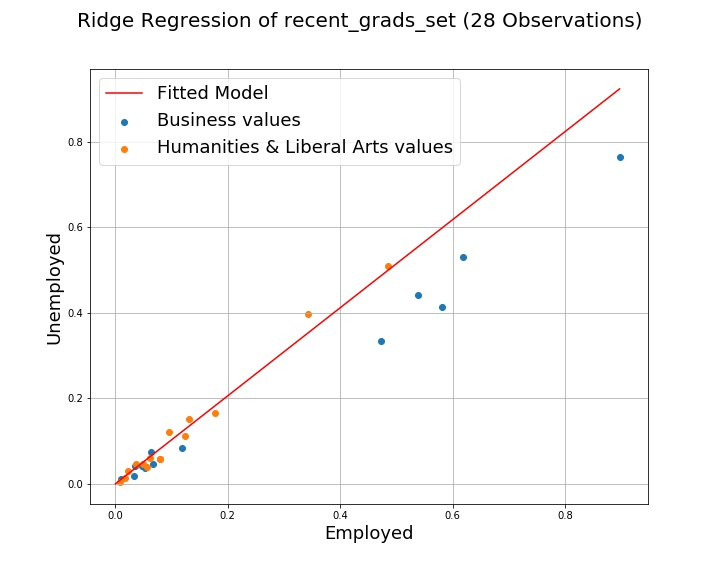
\includegraphics[width=8cm]{ridge_reg_1d_recent_grads_set} As for the mean-squared error and the root-mean-squared error values, the standard regression computed 0.28 and 0.53 while ridge regression calculated 0.25 and 0.50. Unlike the standard and ridge regression models of the generated set of points, there is a noticeable change between both models using the graduate student dataset; the difference being the increase in slope for the line of best, and both the mean-squared error and the root-mean-squared error decreasing by 0.03 points. This means that the ridge regression model is the better model to use, thus far, in prediction.

After the recent graduate student dataset was computed using the lasso regression model, which can be seen below, and then compared to the ridge regression model, it can be seen that there is no apparent change in the slope of the line of best fit, the mean-squared error, nor the root-mean-squared error. 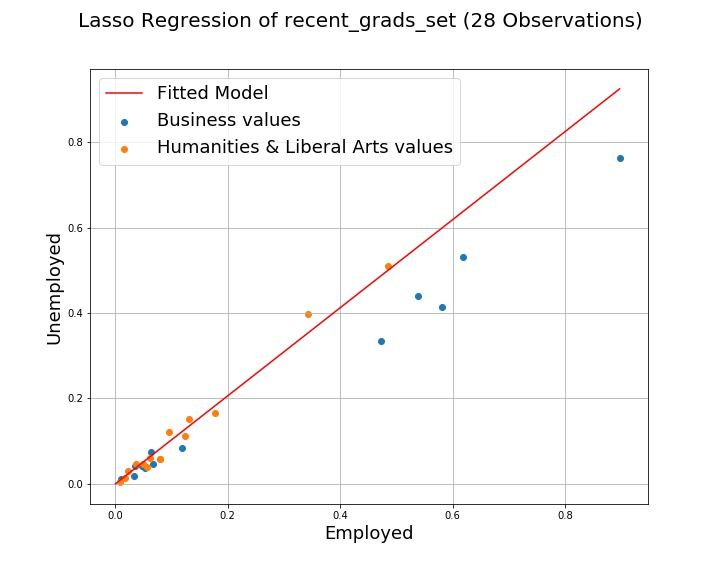
\includegraphics[width=8cm]{lasso_reg_1d_recent_grads_set} This shows that the changes in regularization parameters for ridge and lasso regression result in each of these two regression analyses having similar models and error values.

Now when the recent graduate dataset used the last model, elastic-net regression, the following visualization was constructed: 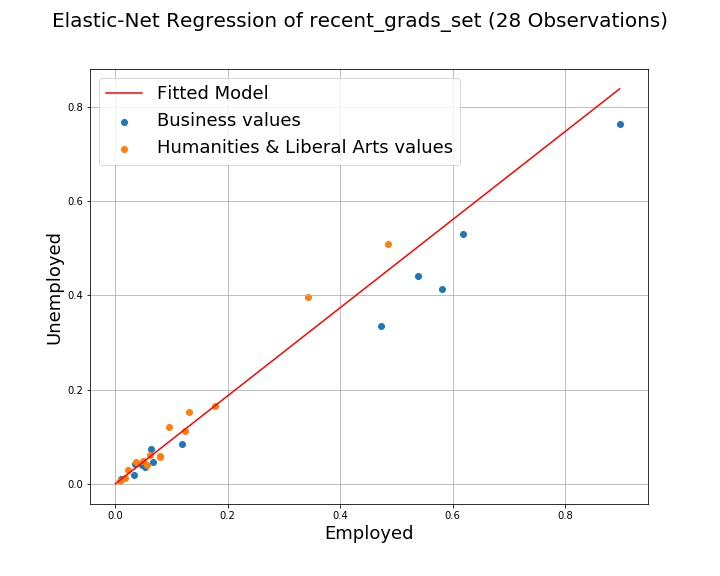
\includegraphics[width=8cm]{en_reg_1d_recent_grads_set} and the calculated mean-squared and root-mean-squared error came to be approximately 0.20 and 0.45; a decrease of about 0.05 points from the error values given in both ridge and lasso regression. Therefore, elastic-net regression has proven itself to be the most optimal approach for finding the regression model and computing prediction values on the recent graduate students dataset.

\subsection{Graduate Student Dataset}
\label{grad}
For the graduate student dataset, the standard regression analysis created the following plot and resulted in a mean-squared error of 0.05 and a root-mean-squared error of 0.22. 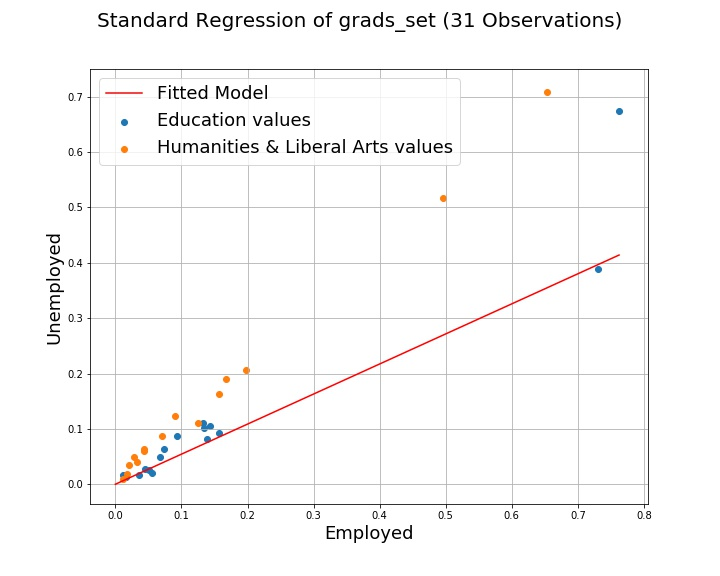
\includegraphics[width=8cm]{std_reg_1d_grads_set} After this, the ridge regression model was fitted for the dataset and this plot: 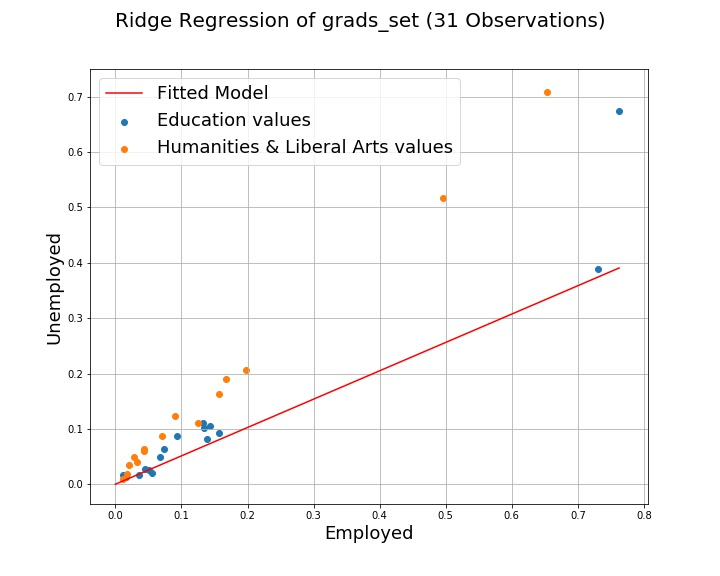
\includegraphics[width=8cm]{ridge_reg_1d_grads_set} was created and featured a MSE value of 0.04 and a RMSE value of 0.20. Notice when the ridge regression is compared to the standard regression, not only are the error values lower, but the slope of the line of best fit also decreases, meaning that the ridge regression model is, so far, the better fitting model for the graduate student dataset.

When the lasso regression analysis is run on the dataset, it results in a similar MSE value as the ridge regression, but the root-mean-squared error for the lasso regression model is slightly lower (by 0.01 points to give an estimation). The lasso regression model also creates the following visualization, which when compared to the ridge regression line of best fit, has a noticeable decrease in slope value. 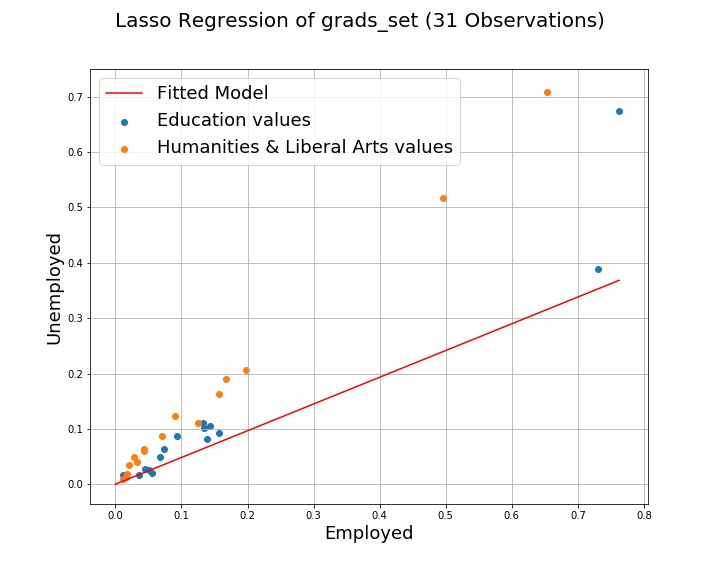
\includegraphics[width=8cm]{lasso_reg_1d_grads_set} With this in mind, while the ridge and lasso regressions are very similar in modeling, the lasso regression proves to be more efficient than the previous models.

Finally, when the elastic-net regression analysis was run on the graduate student dataset, the MSE and RMSE values were calculated to be approximately 0.02 and 0.15 and resulted in the following plot: 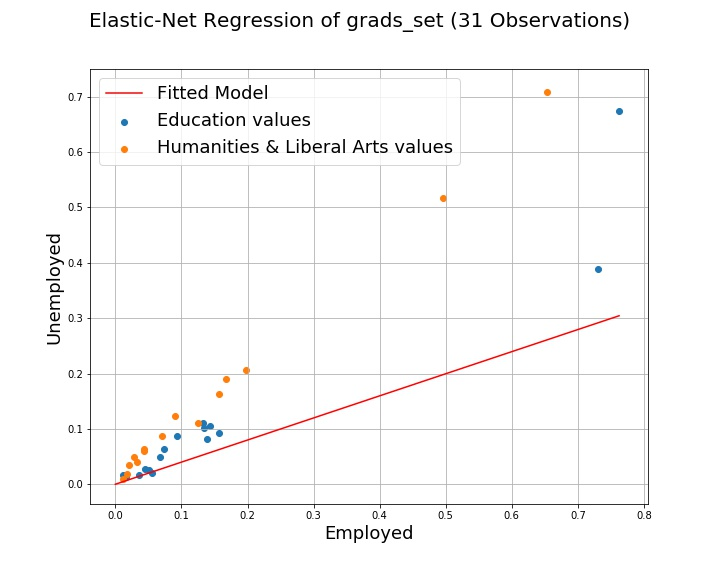
\includegraphics[width=8cm]{en_reg_1d_grads_set} Notice that of all the regression models used on this specific dataset, the elastic-net regression has the lowest slope value and the lowest error values. Therefore, elastic-net regression has once again proven itself to have the best fitting model of all four regression analyses.

\subsection{Regression Model Inference}
\label{reg_summary}
Using the information gathered from running the generated set of points, the recent graduate student dataset and the graduate student dataset, it can be inferred that parameterization will either have no effect on regression models or a significant impact on them. In the case of the generated set of points, the change in parameters did not lead to much progress in optimization which means the results of each type of regression utilized were similar to each other. As for both the datasets about graduate students, it can be seen that using different parameters on the estimate \textit{A} made choosing the best regression model obvious. It also showed that if each regression model has different prediction values, the model with the lowest error will tend to be the one that contains the most regularization parameters.

\section{Network Intrusion Datasets and Random Forest}
An understanding of classification is the next step in comprehending how machine learning works and choosing which techniques are need to find characteristics of data. To do this, one must first know what classification is and how it differs in from regression. In short, classification is a type of supervised learning involves labeling, or classifying, data into different categories so that it becomes less complex to draw conclusions about the traits of said data. The main difference between classification and regression is that regression is about mathematically predicting feature values using continuous data while classification is about predicting the classification category that each piece of data in a discrete set of information belongs to based off its attributes. With this in mind, the classification portion of the assignment can be clearly understood.

In this portion of the experiment, the two datasets featuring captured network traffic will be classified by using the machine learning technique called Random Forest classification. The following steps were in the experiment to identify each data class's traits:
\begin{enumerate}
\item A statistical analysis of the captured network traffic.
\item The preprocessing of data features and feature selection.
\item Applying the Random Forest technique and its evaluation.
\item Reducing the data dimensions to find the most important characteristics of the the data categories.
\end{enumerate}

When the initial statistical analysis on the network intrusion dataset took place, a lot of useful information was gathered that would help in the classification process. According to the computed statistics, there were 25,192 observations in both data sources where all observations were labeled via the twenty-two initial labels describing the network traffic type. Out of the twenty-two labels, there were only two classes in which each label fell into: normal traffic or attack traffic. Using this information, the dataset could be properly identified as reasonably balanced because each dataset an almost equal amount of normal and attack traffic types.

In the preprocessing process of classification, it was decided that only numerical features would be used for labeling, which means all categorical data was excluded. Once the numerical feature columns were selected, quantitative measures were taken to prepare the data for training; this involved extracting the data domain and response set, then normalizing and standardizing the features. At this point, there were thirty-seven standardized, numerical features in the first network intrusion set and thirty-six standardized, numerical features for the second dataset.

After the preprocessing and feature selection steps were finished, the Random Forest technique could now be applied to the data and evaluated. When this was done, it was determined that there might be a slight error in using the Random Forest classification for the data because the Binary-Classification Evaluator and Cross-Validator from PySpark resulted in what seems to be inaccurate test error values for both datasets. Besides this supposed error, finding the most important features in the data was relatively simple and dimensionality reduction was not complex.

Now, the most important features were selected based on the criteria that the accuracy of the column calculated by the Random Forest model had to be greater than the value 0.1. With this criteria in mind, there were only four columns in the \textit{nslkdd-version1.csv} that had significant value in computing classification out of the thirty-seven numerical features used, according to the Random Forest classifier; the sum of the four important features in classification came to be approximately 0.88. In the \textit{nslkdd-version1.csv} file, there was only three numerical features that were considered important out of the thirty-six used in classification and those columns' accuracies summed up to be 0.79. 

\subsection{Random Forest Classification Inference}
\label{class}
Using this knowledge, it can be inferred that if the Random Forest technique was the only classification used on the network intrusion datasets, then these columns may be the only features need to appropriately predict the labels of future observations. Though, with the binary classification evaluator and cross-validation errors being so low, it could be considered unwise to only use Random Forest on the data. To ensure the appropriate feature selection needed for the network intrusion categorization, a better classifier may be required to process the data separately from the Random Forest model.

\section{Results}
In conclusion, the assignment was successful in teaching which supervised learning techniques are useful for certain applications of data. It also demonstrated the importance of preprocessing features and selecting the appropriate features needed in order to make accurate predictions on data. The main lesson learned from the experiment was that it taught how machine learning models and algorithms function function together in order to make certain learning techniques such as regression and classification more suitable for data applications. With all of these in mind, a development for an understanding of how big data and machine learning interact together can be furthered and allows for an enhanced knowledge on the attributes of the field of data science.

\end{document}